\documentclass[11pt, oneside]{article}   	% use "amsart" instead of "article" for AMSLaTeX format
\usepackage{geometry}                		% See geometry.pdf to learn the layout options. There are lots.
\geometry{letterpaper}                   		% ... or a4paper or a5paper or ... 
%\geometry{landscape}                		% Activate for for rotated page geometry
%\usepackage[parfill]{parskip}    		% Activate to begin paragraphs with an empty line rather than an indent
\usepackage{graphicx}				% Use pdf, png, jpg, or eps� with pdflatex; use eps in DVI mode
								% TeX will automatically convert eps --> pdf in pdflatex		
\usepackage{amssymb}
\usepackage{amsmath}
\usepackage{parskip}

\title{Squares Problem}
%\author{The Author}
%\section{}
% \subsection*{R code}
\date{}							% Activate to display a given date or no date

\graphicspath{{/Users/telliott_admin/Dropbox/Tex/png/}}

% \begin{center} 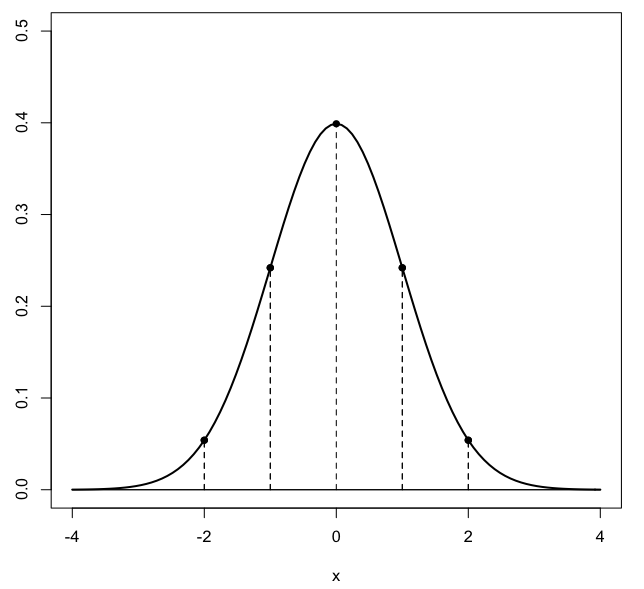
\includegraphics [scale=0.4] {gauss3.png} \end{center}
% \begin{bmatrix} a  &  b \\ c  &  d \end{bmatrix}
% \bigg |_

\begin{document}
\maketitle
\Large
%\noindent
We have the following problem:  place three squares next to each other and draw the lines connecting vertices as shown.  To prove:  angle $a$ is equal to angle $c$
\begin{center} 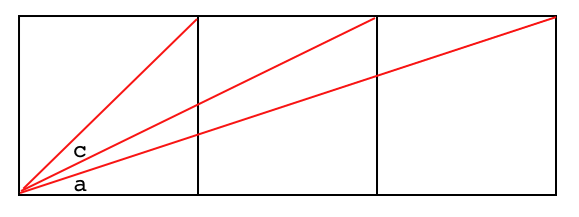
\includegraphics [scale=0.4] {squares_prob1.png} \end{center}
From similar triangles, we recognize that the altitude of the triangle containing $a$ is equal to one-third of the side length, while the triangle containing angle $a+b$ has an altitude one-half of the side length.  Remembering that, we can concentrate on the first square, adding some labels.
\begin{center} 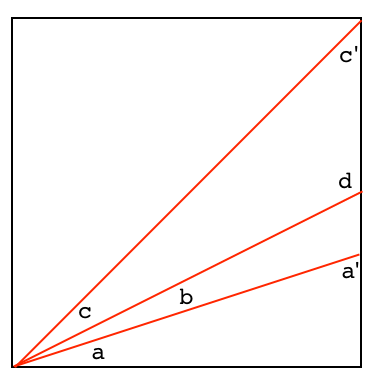
\includegraphics [scale=0.4] {squares_prob2.png} \end{center}
One way to solve this is to do algebra on the angles.
We have the following relationships:
\[ c' = 45 \]
\[ c + 45 + d = 180 \]
\[ a + a'  = 90 \]
\[ a + b  + c = 45 \]
Let's get another copy of the figure
\begin{center} 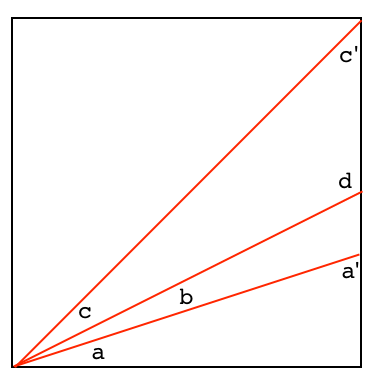
\includegraphics [scale=0.4] {squares_prob2.png} \end{center}
Also, adding up the angles in that inner triangle
\[ b + (180 - d) + (180 - a') = 180 \]
Substituting
\[ (45 - a - c) + (c + 45) + (180 - (90 - a)) = 180 \]
\[ 45 - a - c + c + 45 + 180 - 90 + a = 180 \]
Everything in this equation cancels.  It is no help, and the reason is that we haven't used the information we've been given about the relative heights of the altitudes.

Try again:
\begin{center} 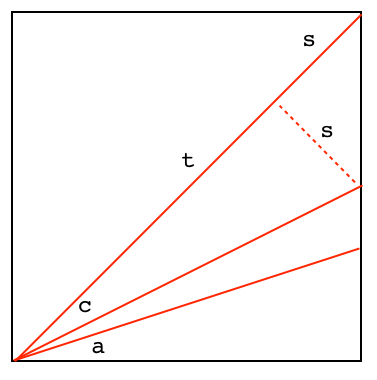
\includegraphics [scale=0.4] {squares_prob3.png} \end{center}
Because the angle at the upper vertex is $45$ degrees, the small triangle is isosceles.  The equal sides are labeled $s$ and the rest of the long side is labeled $t$.  

If the length of the side is scaled to be $1$, then one-half the side length is $1/2$ and
\[ s^2 + s^2 = (\frac{1}{2})^2 = \frac{1}{4} \]
\[ s = \frac{1}{\sqrt{8}} \]

The whole diagonal is $\sqrt{2}$, so
\[ t = \sqrt{2} - s = \sqrt{2} - \frac{1}{\sqrt{8}} = \frac{\sqrt{16}}{\sqrt{8}} - \frac{1}{\sqrt{8}} = \frac{4-1}{\sqrt{8}} = \frac{3}{\sqrt{8}} \]
Then
\[ \tan c = \frac{s}{t} = \frac{1}{3} \]
Way back at the beginning we said that the altitude of the triangle with angle $a$ is one-third the side length so
\[ \tan a = \frac{1/3}{1} = \tan c \]
so $a = c$.

Now, I don't have the original problem statement any more, but as I recall the challenge was to not use trigonometry, just geometry.  And I am not sure how to do that.

\end{document}  